\documentclass[border=3mm,tikz,preview]{standalone}
\usepackage[utf8]{inputenc}
\usepackage{amsmath,amssymb,amsfonts}
\usepackage{graphicx}
\usepackage{tikz}
\usetikzlibrary{shapes.geometric, arrows.meta, positioning, shadows, calc, fit, backgrounds}
\usepackage{xcolor}
\begin{document}

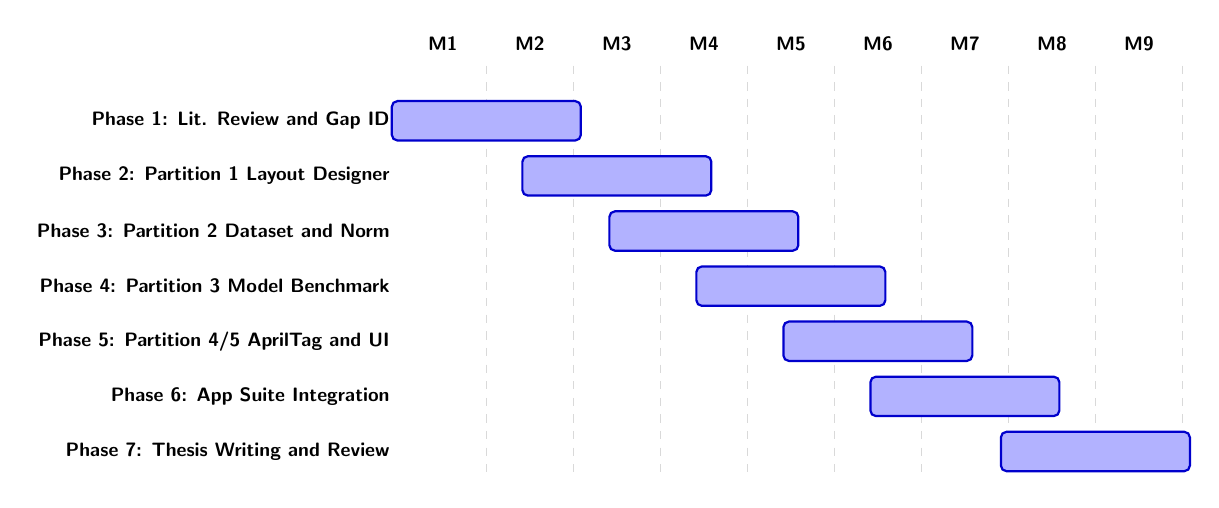
\begin{tikzpicture}[
    xscale=0.85,
    yscale=0.7,
    task/.style={rectangle, draw=blue!80!black, fill=blue!30!white, thick, rounded corners=2pt, minimum height=0.5cm, font=\sffamily\tiny\bfseries},
    gridline/.style={draw=gray!30, dashed}
]

% Grid Lines for Months M1 to M9
\foreach \m [count=\i] in {M1, M2, M3, M4, M5, M6, M7, M8, M9} {
    \draw[gridline] (\i*1.3, 0) -- (\i*1.3, -7.5);
    \node at (\i*1.3 - 0.65, 0.4) [font=\sffamily\scriptsize\bfseries] {\m};
}

% Task Rows
\node [left, font=\sffamily\scriptsize\bfseries] at (0, -1.0) {Phase 1: Lit. Review and Gap ID};
\node [task, minimum width=2.4cm] at (1.3, -1.0) {};

\node [left, font=\sffamily\scriptsize\bfseries] at (0, -2.0) {Phase 2: Partition 1 Layout Designer};
\node [task, minimum width=2.4cm] at (3.25, -2.0) {};

\node [left, font=\sffamily\scriptsize\bfseries] at (0, -3.0) {Phase 3: Partition 2 Dataset and Norm};
\node [task, minimum width=2.4cm] at (4.55, -3.0) {};

\node [left, font=\sffamily\scriptsize\bfseries] at (0, -4.0) {Phase 4: Partition 3 Model Benchmark};
\node [task, minimum width=2.4cm] at (5.85, -4.0) {};

\node [left, font=\sffamily\scriptsize\bfseries] at (0, -5.0) {Phase 5: Partition 4/5 AprilTag and UI};
\node [task, minimum width=2.4cm] at (7.15, -5.0) {};

\node [left, font=\sffamily\scriptsize\bfseries] at (0, -6.0) {Phase 6: App Suite Integration};
\node [task, minimum width=2.4cm] at (8.45, -6.0) {};

\node [left, font=\sffamily\scriptsize\bfseries] at (0, -7.0) {Phase 7: Thesis Writing and Review};
\node [task, minimum width=2.4cm] at (10.4, -7.0) {};

\end{tikzpicture}

\end{document}
